\documentclass{exam}
\usepackage{graphicx}
\begin{document}
\begin{questions}
\question Who is not Cem?\newline
\begin{oneparchoices}
\choice 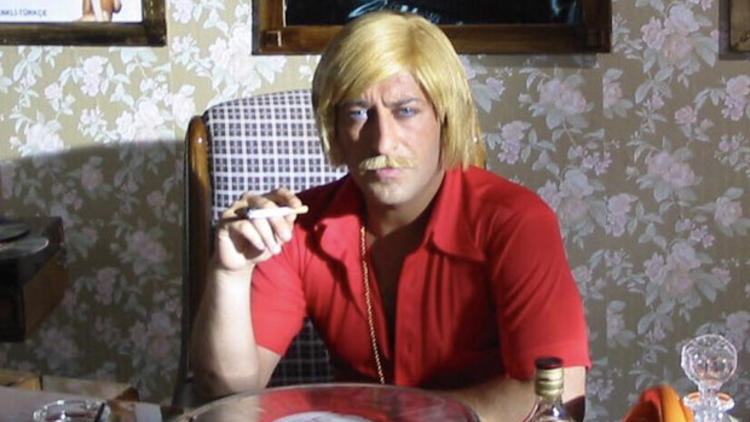
\includegraphics[height=2em]{ersan.jpg}
Ersan Kuneri
\CorrectChoice 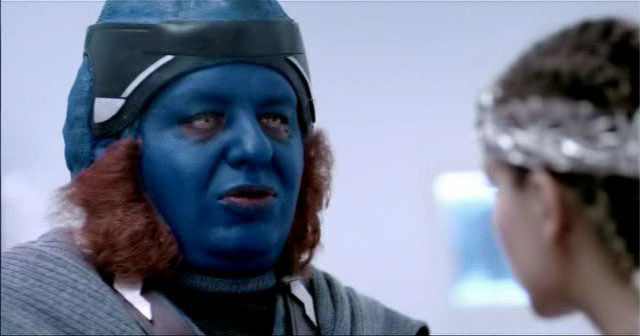
\includegraphics[height=2em]{rendroy2.jpg}
Rendroy
\choice 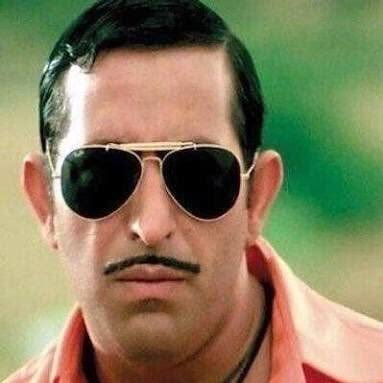
\includegraphics[height=2em]{arifisik.jpg}
Arif Isik
\choice 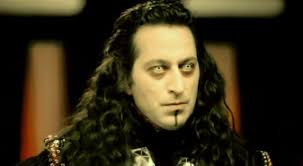
\includegraphics[height=2em]{komutanlogar.jpeg}
Komutan Logar
\end{oneparchoices}
\question HEY SELAM!\newline
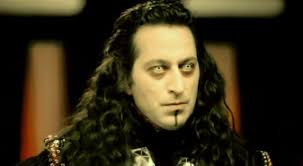
\includegraphics[height=3em]{komutanlogar.jpeg} \newline
\begin{oneparchoices}
\choice 
\includegraphics[height=2em]{faruk.jpg}
Ve tabi ki ben de bir secenegim
\CorrectChoice 
\includegraphics[height=2em]{216.jpg}
Ben de bir secenegim
\choice 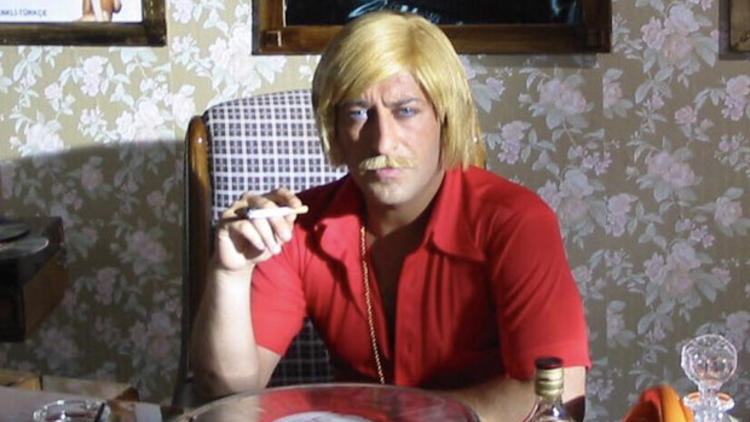
\includegraphics[height=2em]{ersan.jpg}
e ben de oyle
\choice 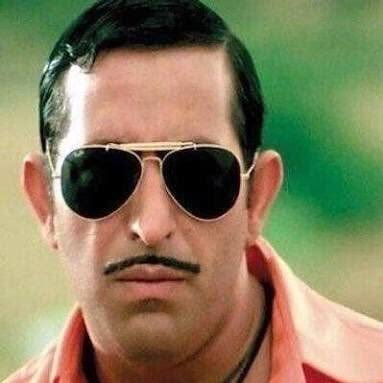
\includegraphics[height=2em]{arifisik.jpg}
Ben bir secenegim
\end{oneparchoices}
\question Komutan Logar bir cisim Yaklasiyor Efendim\newline
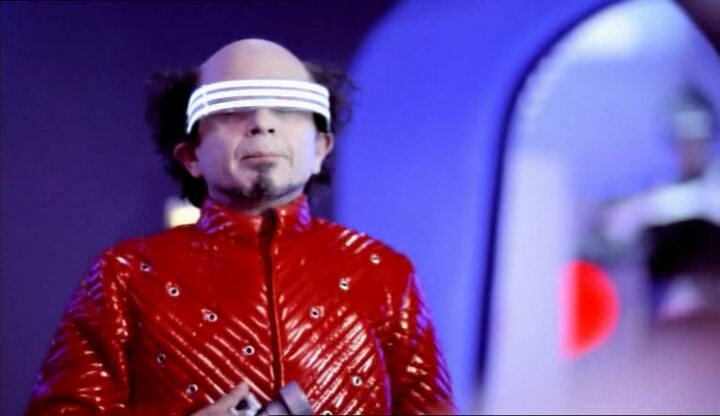
\includegraphics[height=3em]{tihulu.jpeg} \newline
\begin{oneparchoices}
\choice Komutan Logar
\choice Ceku
\choice Mulu
\CorrectChoice Tihulu
\end{oneparchoices}
\question Four Elements\newline
\begin{oneparchoices}
\choice Su-Toprak-Hava-Patates
\choice Ates-Su-Toprak-Hava
\choice Ates-Su-Toprak-Limon
\CorrectChoice Ates-Su-Toprak-Tahta
\end{oneparchoices}
\question Which one of them is true?\newline
\begin{oneparchoices}
\choice 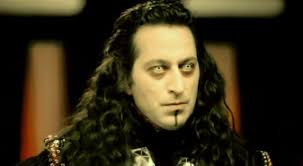
\includegraphics[height=2em]{komutanlogar.jpeg}
\CorrectChoice 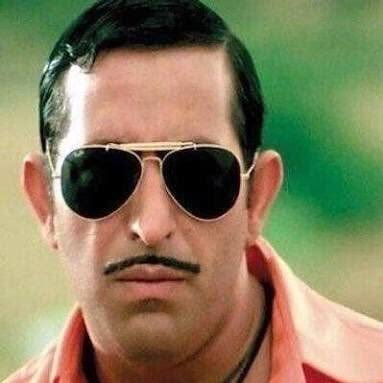
\includegraphics[height=2em]{arifisik.jpg}
\choice 
\includegraphics[height=2em]{faruk.jpg}
\choice 
\includegraphics[height=2em]{216.jpg}
\end{oneparchoices}
\question Deneme Body\newline

\includegraphics[height=3em]{faruk.jpg} \newline
\begin{oneparchoices}
\choice \includegraphics[height=2em]{}
Choice3
\choice \includegraphics[height=2em]{}
Choice4
\choice 
\includegraphics[height=2em]{216.jpg}
Choice2
\CorrectChoice \includegraphics[height=2em]{}
Choice1
\end{oneparchoices}
\question Who Is thisadfadasadsafsdfsadafsadfsa\newline
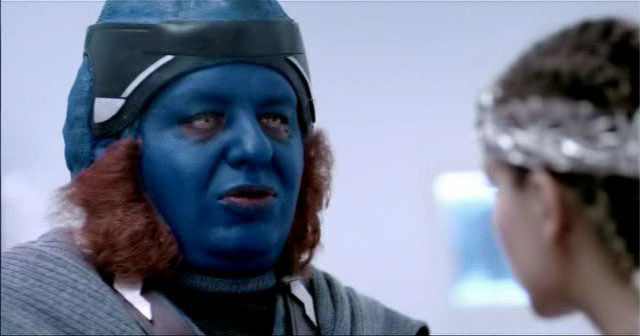
\includegraphics[height=3em]{rendroy2.jpg} \newline
\begin{oneparchoices}
\CorrectChoice Rendroy
\choice Amir Tocha
\CorrectChoice ANOTHERDEGISIM
\choice Deneme Method
\end{oneparchoices}
\end{questions}
\end{document}